To add two numbers we need an addition processes that mimics the behavior of arithmetic circuits for adding two bits binary numbers shown in 
\refFig{tra_adder_circuit}.
\refFig{tra_addition} shows visualization of the addition process and the ABC code.
The full implementation of $Add$ processes can be found in the appendix.
\begin{figure}[H]%
\centering
\fbox{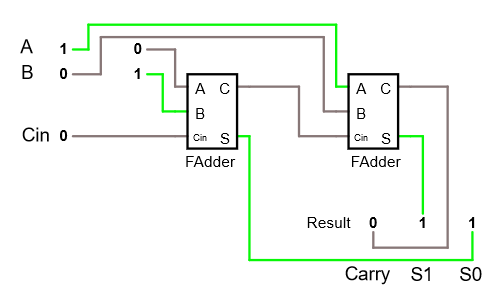
\includegraphics[keepaspectratio]{./images/transformational_semantics_of_oz/adder_circuit.png}}
\caption{Adder circuit}
\label{tra_adder_circuit}%
\end{figure}


\begin{figure}[H]%
\centering
\hspace{\fill}
\subcaptionbox{Before addition.}{\fbox{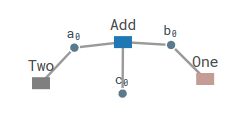
\includegraphics[keepaspectratio,width=0.45\textwidth]{./images/transformational_semantics_of_oz/add_before.png}}}%
\hspace{1em}%
\subcaptionbox{After addition.}{\fbox{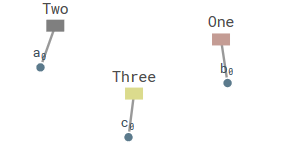
\includegraphics[keepaspectratio,width=0.45\textwidth]{./images/transformational_semantics_of_oz/add_after.png}}}%
\vspace{2em}
\subcaptionbox{Abc code.}{\fbox{$(\ \widehat{}\ \text{a,b,c}\ )\ (\ \text{Two}(\text{a})\ \mid\ \ \text{One}(\text{b})\ \mid\ \ \text{Add}(\text{a,b,c})\ )$}}%
\caption{Addition as a process}
\label{tra_addition}%
\end{figure}
